\chapter{Results\label{chap:Results}}
This chapter describes the results of the two experiments conducted for this thesis.  Post\-/hoc analyses that help to clarify and explain the results are described in Chapter~\ref{chap:Discussion}. 

\section{Experiment 1}
Experiment~1 tests the role of prosody in intelligibility, by comparing mean sentence scores for unmodified talkers against resynthesized stimuli with prosodic replacement.  A quartile analysis indicated a significant improvement in performance between the first and last quartiles (\textit{t}=−3.016 on 709.3 degrees of freedom, \textit{p}<0.01; see Figure~\ref{fig:ExpOneQuartile}).  The magnitude of the difference between the first and fourth quartiles is approximately 0.4 keywords.

\begin{figure}[htbp]
	\begin{centering}
	\includegraphics{figures/results/ExpOneQuartileBarplot.eps}
	\caption[Mean sentence scores by quartile for Experiment~1]{Mean sentence scores by quartile for Experiment~1.  Error bars are ±1 standard error.\label{fig:ExpOneQuartile}}
	\end{centering}
\end{figure}

The mean sentence score for each talker across listeners is shown in Figure~\ref{fig:ExpOneBarplot}.  Darker bars indicate unmodified stimuli, while light bars represent resynthesized stimuli.  It is noteworthy that not all resynthesized stimuli have lower mean scores compared to their unmodified counterparts, suggesting that distortion due to the resynthesis process was relatively minimal.  This is likely due to several factors; one is probably the painstaking hand\-/correction of the pulse marks during stimulus preparation, which ensured consistent phase of the \fo{} epochs throughout voiced spans of speech.  Another possible explanation for the low levels of distortion is the choice to maintain each talker’s natural mean pitch on each sentence, and map only the {\emph shape} of the pitch contour of the prosodic donor during resynthesis.  

With regard to Research Question~1 — \emph{how does prosody relate to intelligibility?} — a complex picture emerges.  Talker~\ac{b} suffers dramatically when his prosody is replaced, whereas Talker~\ac{c} is unchanged or slightly improved, and Talker~\ac{a} is unchanged or slightly worsened.  One possible explanation for these results is to postulate that Talker~\ac{a}, despite being highly intelligible, does not have especially good prosody, evidenced in particular by the fact that scores for Talker~\ac{ca} are lower than the scores for Talker~\ac{cb}.  On the same grounds, and on the additional observation that scores for Talker~\ac{ab} are greater than for Talker~\ac{ac}, we might conclude that Talker~\ac{b} has more intelligible prosody than the other two talkers, and his middling base intelligibility scores are due to segmental factors.

\begin{figure}
	\begin{centering}
	\includegraphics{figures/results/ExpOneBarplot.eps}
	\caption[Barplot of mean sentence scores for Experiment~1]{Barplot of mean sentence scores for Experiment~1.  Error bars are ±1 standard error; lighter colors indicate resynthesized talkers, with the second letter indicating the prosodic donor (see Section~\ref{sec:ExpDesign} for full explanation of talker codes).  Similar hues indicate shared segmental donors.\label{fig:ExpOneBarplot}}
	\end{centering}
\end{figure}

With regard to the question of whether low\-/intelligibility talkers can be made more intelligible through prosody alone, it would appear that the answer is “yes”: Talker~\ac{cb} appears to have higher scores than Talker~\ac{c}, despite the likelihood that Talker~\ac{cb}’s recordings suffer some amount of distortion from the resynthesis process, however small.  In other words, any degradation due to resynthesis seems to have been more than overcome by the benefit of having Talker~\ac{b}’s prosody mapped onto Talker~\ac{c}’s signal.

\subsection{Experiment~1 statistical model}
To further probe these results, the scores were submitted to a mixed\-/effects linear regression model, shown here:%in Equation~\ref{eq:ExpOneMM}:

\noindent{\small \inlinecode lmer(sentScore\textasciitilde resynth+segDonor+proDonor+trial+(1|listener)+(1|sentence))}
%\begin{equation}\label{eq:ExpOneMM}
%	\text{{\small \inlinecode lmer(sentScore\textasciitilde resynth+segDonor+proDonor+(1|listener)+(1|sentence), data=allData)}}
%\end{equation}

In this model, {\inlinecode sentScore} is the number of keywords correct (0–5), {\inlinecode resynth} is a boolean variable that is true for Talkers~\ac{ab}, \ac{ac}, \ac{ba}, \ac{bc}, \ac{ca} and~\ac{cb}, and {\inlinecode segDonor} and {\inlinecode proDonor} are three\-/level factors indicating the talker in the target signal and the talker from whom the prosodic information was drawn, respectively.  For the unmodified original recordings, {\inlinecode segDonor} and {\inlinecode proDonor} are defined as the talker himself, even though those recordings were not resynthesized.  The effect of task familiarization seen in Figure~\ref{fig:ExpOneQuartile} is accounted for by the fixed\-/effect predictor {\inlinecode trial} (a numeric value ranging from 1–90).

%A summary of the model shown in Equation~\ref{eq:ExpOneMM} 
A summary of fixed\-/effects predictors for this model is given in Table~\ref{tab:ExpOneFixedEff}.  All fixed\-/effects predictors were significantly different from zero, and there was no evidence of correlation of fixed effects (correlation coefficients all less than 0.1; not shown).  The baseline condition is Talker~\ac{a}, with a value at the intercept of about 4.1 words correct.  The coefficients reveal similar patterns to those seen in Figure~\ref{fig:ExpOneBarplot}: firstly, the model supports the interpretation that Talker~\ac{b} has the most intelligible prosody.  Having the prosody of Talker~\ac{b} represents a net gain of 0.3 words correct over the prosody of Talker~\ac{a}, whereas having the prosody of Talker~\ac{c} represents a net loss of more than 0.6 words correct compared to Talker~\ac{a}.  The model also supports the idea that Talker~\ac{a}’s intelligibility stems in large part from non\=/prosodic factors, given that the other levels of {\inlinecode segDonor} both have strongly negative coefficients.  The estimated degradation due to resynthesis is about −0.7 keywords correct.  Because trial was a continuous variable ranging from 1–90, the coefficient for the effect of trial is misleadingly small; the predicted difference between the first and the last trial due to listener adaptation to the task is actually 90×0.005549, or 0.5 keywords.

\begin{table}
	\caption[Experiment~1 statistical model: Fixed effects]{Summary of fixed effect predictors in the statistical model of Experiment~1.  \textit{s}: standard error of the coefficient estimate; \textit{t}: \textit{t}\=/value of coefficient estimate; \textit{p}: \textit{p}\=/value of coefficient estimate (calculated via \ac{mcmc}).\label{tab:ExpOneFixedEff}}
	\centering
	\begin{tabu} spread 1em {Xrcrc}
		\toprule
		\multicolumn{5}{l}{Summary of fixed effects (N=1440; log-likelihood=−2551)}\\
		\rowfont\bfseries
		\multicolumn{1}{l}{Predictor} & \multicolumn{1}{c}{Coefficient} & \textit{s} & \multicolumn{1}{c}{\itshape t} & \textit{p}\\
		\midrule
		Intercept         &  4.132 & (0.145) &  28.44 & <10⁻¹⁶\\
		resynth = TRUE    & −0.662 & (0.077) &  −8.63 & <10⁻¹⁶\\
		segDonor = \ac{b} & −1.673 & (0.089) & −18.86 & <10⁻¹⁶\\
		segDonor = \ac{c} & −1.278 & (0.089) & −14.31 & <10⁻¹⁶\\
		proDonor = \ac{b} &  0.307 & (0.088) &   3.48 & <10⁻³\\
		proDonor = \ac{c} & −0.646 & (0.088) &  −7.36 & <10⁻¹²\\
		trial             &  0.006 & (0.001) &   4.02 & <10⁻⁴\\
		\bottomrule
	\end{tabu}
\end{table}

A summary of the random effects in the model for Experiment~1 are shown in Table~\ref{tab:ExpOneRandomEff}.  The results here are not unexpected: the variance in intercepts due to particular listeners doing systematically better or worse on the task is only about 2\% of the total residual variance.  This suggests that, by and large, all listeners were performing equally well on the task.  The variance in intercepts due to varying difficulty of particular sentences is somewhat larger (about 22\% of the total residual variance, or a standard deviation of 0.7 keywords correct),\footnotemark{} suggesting that there was indeed some value in modeling the sentences as varying in their difficulty (cf. the discussion of scoring in Section~\ref{sec:Scoring}).
\footnotetext{The \ac{mcmc} estimate for variability due to listener is in close agreement with the fitted model.  The \ac{mcmc} estimate for variability due to sentence is slightly smaller than the value in the fitted model, at 16\% of the total variance (\vs\ 22\%), with a standard deviation for sentence of about 0.6 keywords (\vs\ 0.7).}

\begin{table}
	\caption[Experiment~1 statistical model: Random effects]{Summary of random effects in the statistical model of Experiment~1.  \textit{s}²: estimated variance; \textit{s}: standard error; \ac{hpd}: highest posterior density interval.\label{tab:ExpOneRandomEff}}
	\centering
	\begin{tabu} spread 1em {Xcccc}
		\toprule
		\multicolumn{3}{l}{Summary of random effects} & \multicolumn{2}{c}{\bfseries \ac{mcmc} (nsim=10\thinspace000)}\\ 
		\cmidrule{4-5}
		\rowfont\bfseries
		Group & \textit{s}² & \textit{s} & mean & 95\% \ac{hpd}\\
		\midrule
		Sentence (intercept) & 0.506 & 0.711 & 0.600 & (0.498~~0.700)\\
		Listener (intercept) & 0.043 & 0.207 & 0.220 & (0.100~~0.346)\\
		Residual             & 1.767 & 1.329 & 1.344 & (1.294~~1.396)\\
		\bottomrule
	\end{tabu}
\end{table}

\section{Experiment 2}
Experiment~2 tests the role of prosody in the familiar talker advantage, by comparing mean sentence scores for various talkers across two groups of listeners: those trained on one of the test talkers (Talker~\ac{c}), and those trained on a control talker (Talker~\ac{d}).  The first question to be addressed is whether the training phase was in fact effective for both groups of listeners.   

\begin{figure}[htbp]
	\begin{centering}
	\includegraphics{figures/results/ExpTwoOctileBarplot.eps}
	\caption[Quartile analysis of Experiment~2 training and testing phases]{Quartile analysis of training and testing phases in Experiment~2 (all listeners combined).  Significant improvement is seen during the training phase, but not during testing.\label{fig:ExpTwoOctileBarplot}}
	\end{centering}
\end{figure}

Across all listeners, performance shows an upward trend in mean sentence score across training quartiles (\textit{t}=−4.00 on 878.3 degrees of freedom, \textit{p}<0.0001), but no significant changes across quartiles of the testing phase (see Figure~\ref{fig:ExpTwoOctileBarplot}).  This suggests that training was successful in general, and that any familiarization effects were complete before the start of the testing phase.

Considering the control and experimental listener groups separately, both show an upward trend in mean sentence score across training quartiles, and \textit{t}\=/tests performed on the first and fourth quartile of each group show a statistically significant improvement in both groups of listeners (control group: \textit{t}=−2.898 on 437.2 degrees of freedom, \textit{p}<0.01; experimental group: \textit{t}=−2.816 on 438.1 degrees of freedom, \textit{p}<0.01; see Figure~\ref{fig:Quartile}).  The magnitude of the improvement differs slightly between the control group (0.50 keywords) and the experimental group (0.38 keywords).  

\begin{figure}
	\begin{centering}
	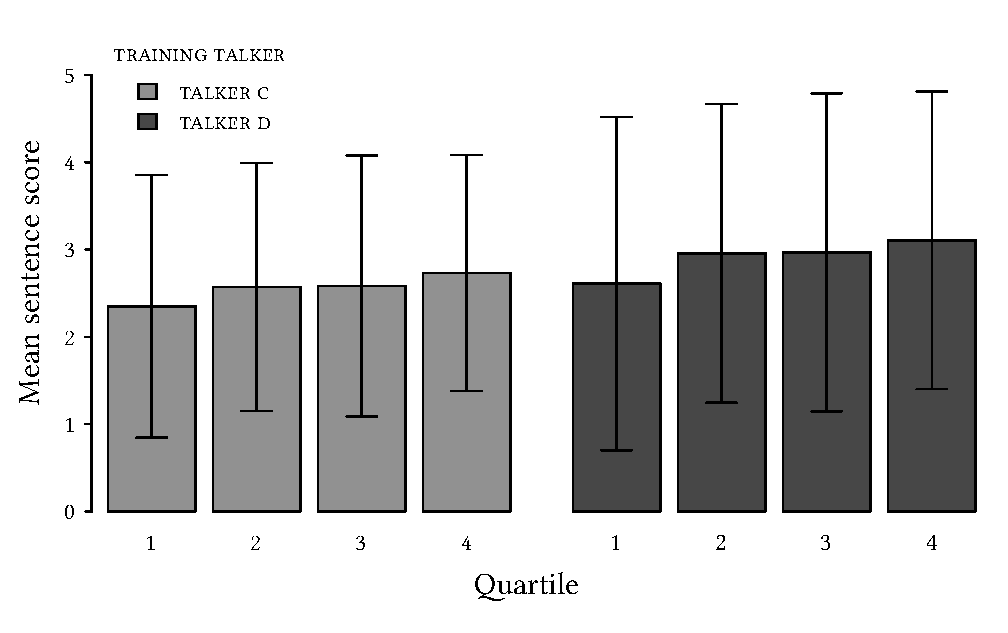
\includegraphics{figures/results/QuartileBarplot.eps}
	\caption[Quartile analysis of training phase in Experiment~2]{Quartile analysis of training phase in Experiment~2.  Improvement is seen during training for both the control group (trained on Talker~\ac{d}) and the experimental group (trained on Talker~\ac{c}).  The adaptation in the experimental group appears not to have persisted through the testing phase.\label{fig:Quartile}}
	\end{centering}
\end{figure}

For the experimental group, it appears that familiarization with Talker~\ac{c} during training did not confer an advantage on Talker~\ac{c} during testing (compare the last quartile of the training phase to the score on Talker~\ac{c} during the testing phase in Figure~\ref{fig:Quartile}).  %\footnotemark{}
%\footnotetext{This is true at least for the listeners trained on Talker~\ac{c}.  Listeners trained on Talker~\ac{d} did not hear their training talker during the testing phase, so it is unknown whether any adaptation was retained during testing.  Presumably, however, any such adaptation would have had little effect on performance when listening to Talkers~\ac{a}, \ac{b}, or \ac{c}.}
In light of this, it is perhaps unsurprising that training did not confer a reliable perceptual advantage on test stimuli resynthesized to have the training talker’s prosody; this is seen in the barplot of mean sentence scores for the testing phase of Experiment~2 (Figure~\ref{fig:ExpTwoBarplot}).  Even without controlling for multiple comparisons, none of the \textit{t}\=/tests comparing the experimental and control groups within talker are significant, suggesting that there was no familiar talker advantage enjoyed by the experimental group.  If there had been a familiar talker advantage, we would have expected the colored bars to be higher than their corresponding grey bars for Talker~\ac{c}, and perhaps for Talkers~\ac{ca}, \ac{cb}, \ac{ac} and \ac{bc} (depending on whether and how the advantage extended to resynthesized talkers).

\begin{figure}
	\begin{centering}
	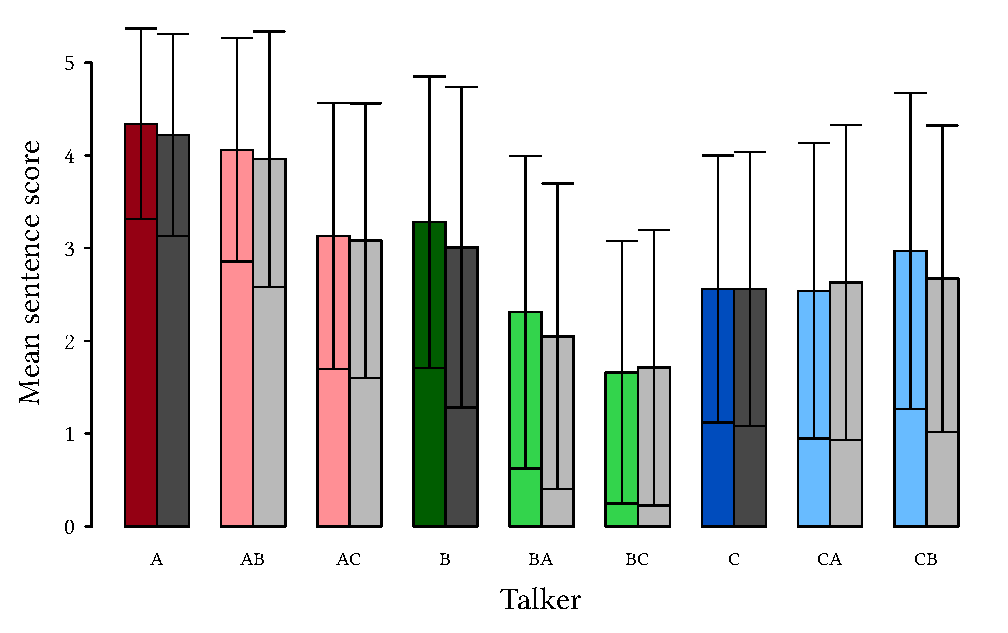
\includegraphics{figures/results/ExpTwoBarplot.eps}
	\caption[Barplot of mean sentence scores for Experiment~2]{Barplot of mean sentence scores for Experiment~2.  Error bars are ±1 standard error.  Colored bars indicate the experimental group; grayscale bars the control group.  Lighter colors indicate resynthesized talkers, and similar hues indicate shared segmental donors.\label{fig:ExpTwoBarplot}}
	\end{centering}
\end{figure}

\subsection{Experiment~2 statistical model}
Full results of the statistical model for Experiment~2 are shown in Table~\ref{tab:ExpTwoFixedEff}.  Predictor codes are the same as in the model for Experiment~1, with the addition of Boolean variables {\inlinecode segTrain} (indicating match between the training talker and the segmental donor of the test stimulus) and {\inlinecode proTrain} (indicating match between the training talker and the prosodic donor of the test stimulus).  Unlike the model for Experiment~1, there is no significant effect for {\inlinecode trial} (unsurprising given Figure~\ref{fig:ExpTwoOctileBarplot}).  Aside from the lack of effect for {\inlinecode trial} and the two additional non\=/significant predictors {\inlinecode segTrain} and {\inlinecode proTrain}, the model is nearly identical to the model for Experiment~1; the magnitude, direction, and significance of the other fixed\-/effect predictors are all unchanged from Experiment~1.

\begin{table}
	\caption[Experiment~2 statistical model: Fixed effects]{Summary of fixed effect predictors in the statistical model of Experiment~2.  \textit{s}: standard error of the coefficient estimate; \textit{t}: \textit{t}\=/value of coefficient estimate; \textit{p}: \textit{p}\=/value of coefficient estimate (calculated via \ac{mcmc}).\label{tab:ExpTwoFixedEff}}
	\centering
	\begin{tabu} spread 1em {Xrcrc}
		\toprule
		\multicolumn{5}{l}{Summary of fixed effects (N=1800; log-likelihood=−3103)}\\
		\rowfont\bfseries
		\multicolumn{1}{l}{Predictor} & \multicolumn{1}{c}{Coefficient} & \textit{s} & \multicolumn{1}{c}{\itshape t} & \textit{p}\\
		\midrule
		Intercept	      &  4.366 & (0.139) &  31.50 & <10⁻¹⁶\\
		resynth = TRUE    & −0.603 & (0.066) &  −9.15 & <10⁻¹⁶\\
		segDonor = \ac{b} & −1.466 & (0.075) & −19.42 & <10⁻¹⁶\\
		segDonor = \ac{c} & −1.159 & (0.098) & −11.80 & <10⁻¹⁶\\
		proDonor = \ac{b} &  0.270 & (0.075) &   3.60 & <10⁻³\\
		proDonor = \ac{c} & −0.584 & (0.098) &  −5.95 & <10⁻⁸\\
		segTrain = TRUE   &  0.008 & (0.125) &   0.06 & 0.95\\
		proTrain = TRUE   & −0.117 & (0.125) &  −0.94 & 0.35\\
		trial             & −0.001 & (0.001) &  −0.64 & 0.53\\
		\bottomrule
	\end{tabu}
\end{table}

A summary of the random effects in the model of Experiment~2 are shown in Table~\ref{tab:ExpTwoRandomEff}.  The results are also very similar to Experiment~1, with estimates of listener accounting for about 4\% of the total unexplained variability (with a standard deviation of 0.3 keywords) and sentence accounting for about 24\% of total unexplained variability (with a standard deviation of about 0.7 keywords).\footnotemark{}

\footnotetext{Again, \ac{mcmc} estimates for the effect of sentence were slightly smaller than the fitted model (18\% \vs\ 24\%), and there was close agreement between the two for the effect of listener.}

\begin{table}
	\caption[Experiment~2 statistical model: Random effects]{Summary of random effects in the statistical model of Experiment~2.  \textit{s}²: estimated variance; \textit{s}: standard error; \ac{hpd}: highest posterior density interval.\label{tab:ExpTwoRandomEff}}
	\centering
	\begin{tabu} spread 1em {Xcccc}
		\toprule
		\multicolumn{3}{l}{Summary of random effects} & \multicolumn{2}{c}{\bfseries \ac{mcmc} (nsim=10\thinspace000)}\\ 
		\cmidrule{4-5}
		\rowfont\bfseries
		Group & \textit{s}² & \textit{s} & mean & 95\% \ac{hpd}\\
		\midrule
		Sentence (intercept) & 0.537 & 0.733 & 0.617 & (0.526~~0.712)\\
		Listener (intercept) & 0.083 & 0.288 & 0.297 & (0.192~~0.425)\\
		Residual             & 1.617 & 1.271 & 1.285 & (1.242~~1.329)\\
		\bottomrule
	\end{tabu}
\end{table}

\section{Post-hoc analyses}
Overall, the statistical models for Experiments~1 and~2 support the view that both prosodic and non\=/prosodic factors contribute to differences in the intelligibility of talkers.  To better understand these results, a variety of acoustic measurements were performed on the stimuli, in hopes of identifying the acoustic dimensions that underlie the effects seen in the statistical models.  The measures are broadly divided into segmental measures (presence of stop release bursts, properties of the vowel space) and prosodic measures (mean pitch range, pitch velocity, intensity velocity, and speech rate).

\subsection{Segmental measures}
TODO: INSERT DATA ON STOP RELEASE BURSTS HERE.
% TODO: post hoc: count release bursts?

In order to remain agnostic about which measurements best characterize overall vowel space size, several different metrics were calculated, based on hand\-/measurements of 5 tokens per vowel per talker for the ten vowels /i ɪ e ɛ æ ɑ o ʊ u ʌ/.  Measured vowels were drawn from keywords in positions throughout the sentence, with a preference for vowels with obstruent flanking consonants to avoid coloring by adjacent nasals, rhotics, or laterals.  These hand\-/measured formant values were converted using the bark transform \citep{bark} prior to further analysis.

Five measures of vowel space size were calculated from the formant data: F1 and F2 ranges, mean Euclidean distance from the center of the vowel space \citep[cf.][]{BradlowEtAl1996}, area of the vowel polygon based on phonemic means \citep[cf.][]{BradlowEtAl1996, Neel2008}, and area of the convex hull encompassing all vowel tokens.  In addition, two measures related to the composition of the vowel space were also calculated: total repulsive force of the vowel system \citep[cf.][]{LiljencrantsLindblom1972, Wright2004a} and mean vowel cluster size (area of the ellipse along a bivariate normal density contour, encompassing 68.27\% of the data points — equivalent to ±1 standard deviation from the bivariate mean).  Repulsive force (sometimes called “total energy”) was calculated as the sum of inverse squared distances between all pairs of vowel tokens not belonging to the same phoneme, as in Equation~\ref{eq:force} (where /i/ and /j/ represent the phonemic categories of the vowel tokens being compared, and \textit{r} is the Euclidean distance formula).  This measures the degree to which neighboring vowel phonemes in a system encroach on one another, with higher values of repulsive force corresponding to greater degrees of phoneme overlap or encroachment.  The calculation seen here differs from both \citealt{LiljencrantsLindblom1972} and \citealt{Wright2004a} in calculating force based on individual vowel tokens rather than mean values for each vowel.

\begin{equation}\label{eq:force}
	\sum_{i=1}^{n-1} \sum_{j=i+1}^{n} \frac{1}{r_{ij}^2} \text{, /i/ ≠ /j/}
\end{equation}

\subsection{Prosodic measures}
To quantify variation in talkers’ use of duration, speech rate was calculated (measured in syllables/second).  Because stimuli were \ac{rms} normalized, mean intensity across stimuli is identical, but the mean rate of change of intensity (“intensity velocity”) was calculated for each stimulus and averaged within talkers, in hopes of capturing a talker’s tendency to “trail off” at the ends of utterances, or conversely to maintain a more consistent level across all the keywords in the sentence.  To quantify pitch, the hand\-/corrected pitch tracks for the 90 test sentences were used to calculate average \fo{} range magnitude, as well as the mean rate of change of \fo{} (“pitch velocity”) and the mean absolute value of rate of change in \fo{} (“pitch dynamicity”).
%\footnotetext{The choice to use mean size of pitch range rather than absolute pitch range was motivated by the fact that a given sentence may be uttered in a fairly monotone fashion even by a talker that has a large overall pitch range.  Thus we reason that a talker’s \textit{typical} range across utterances is more indicative of their linguistic use of pitch than their \textit{potential} or \textit{maximal} range.}

%\subsection{Principal components analysis}
%The various acoustic measures described above are in many cases highly correlated with one another
TODO: DESCRIBE P.C.A. \& OTHER POST-HOC MODELS.
% TODO: Description of principal components analysis for predictor selection.
% TODO: Description of acoustic model of intelligibility?  
% TODO: check mismatch between binary and continuous models for experiment 2
